\section{The Riemann Integral}

\begin{definition}
Let $I = [a, b]$, where $a$ and $b$ are real numbers, be a subset of $\mathbb{R}$ and let 
\begin{align*}
    P = \{x_{0}, x_{1}, x_{2}, ..., x_{n-1}, x_{n}\} \hspace{20pt} \text{such that} \hspace{20pt} a = x_{0} < x_{1} < x_{2} < \cdots < x_{n-1} < x_{n} = b
\end{align*}
be a finite subset of numbers contained in $I$. Take each member $x_{i}$ of $P$ and use it to create a sub-interval $I_{i}$ of $I$, such that the union of these sub-intervals is $I$, as follows
\begin{align*}
    I_{0} = [x_{0}, x_{1}) \hspace{20pt} I_{1} = [x_{1}, x_{2})& \hspace{20pt} \cdots \hspace{20pt} I_{n-2} = [x_{n-2}, x_{n-1}) \hspace{20pt} I_{n-1} = [x_{n-1}, x_{n}]\\[2ex]
    &I = I_{0} \cup I_{1} \cup I_{2} \cup \cdots \cup I_{n-2} \cup I_{n-1}
\end{align*}
From each $I_{i}$, choose a number $t_{i}$. We call the following set of ordered pairs a tagged partition
\begin{align*}
    \dot P = \{ \hspace{4pt} ( \hspace{4pt} [x_{i}, x_{i+1}), t_{i} \hspace{4pt} ) \hspace{4pt}\}_{i = 0}^{n-2} \hspace{10pt} \cup \hspace{10pt} \{ \hspace{4pt} ( \hspace{4pt} [x_{n-1}, x_{n}], t_{n-1} \hspace{4pt} ) \hspace{4pt} \}
\end{align*}
\end{definition}

\begin{definition}
The norm of a tagged partition is defined as
\begin{align*}
    \lvert \lvert \dot P \rvert \rvert = \max \{x_{1} - x_{0}, x_{2} - x_{1}, \cdots , x_{n-1} - x_{n-2}, x_{n} - x_{n-1}\}
\end{align*}
\end{definition}

\begin{definition}
A function $f$ on $I=[a, b]$ is said to be Riemann integrable on $[a, b]$ if there exists a real number $L$ such that for every $\epsilon > 0$ there exists a $\delta > 0$ satisfying the following
\begin{align*}
    &\text{whenever} \hspace{4pt} \dot P \hspace{4pt} \text{is a tagged partition of $[a, b]$}\\[2ex]
    &\text{if} \hspace{20pt} \lvert \lvert \dot P \rvert \rvert < \delta \hspace{20pt} \text{then} \hspace{20pt} \Big\lvert \sum_{i=0}^{n-1} f(t_{i})(x_{i+1} - x_{i}) - L \Big\rvert < \epsilon  
\end{align*}
For this course, we will use the following notation for $L$
\begin{align*}
    L = \int_{a}^{b} f(x) dx
\end{align*}
\end{definition}

\begin{example}
This is an example of a Riemann sum. There are infinitely many tagged partitions we could use for any example, all of which are merely an approximation of the integral of the function, except in the limit. We've chosen one that demonstrates the flexibility of these partitions. Notice that the widths of the rectangles are visibly different, and notice the visible difference in where $t_{i}$ is positioned for each interval. This particular partition for the function $f$ can be written as
\begin{align*}
    \dot P = \{ \hspace{4pt} ( \hspace{4pt} [x_{i}, x_{i+1}), t_{i} \hspace{4pt} ) \hspace{4pt} \}_{i = 0}^{6} \hspace{10pt} \cup \hspace{10pt} \{ \hspace{4pt} ( \hspace{4pt} [x_{7}, x_{8}], t_{7} \hspace{4pt} ) \hspace{4pt} \} \hspace{20pt} \text{where} \hspace{20pt} f(x) = \cos x \hspace{20pt} x \in [0, 1]  
\end{align*}
So, for our partition, we have the endpoints
\begin{align*}
    x_{0} = 0 \hspace{20pt} \text{and} \hspace{20pt} x_{8} = 1
\end{align*}
\resizebox{30em}{30em}{%
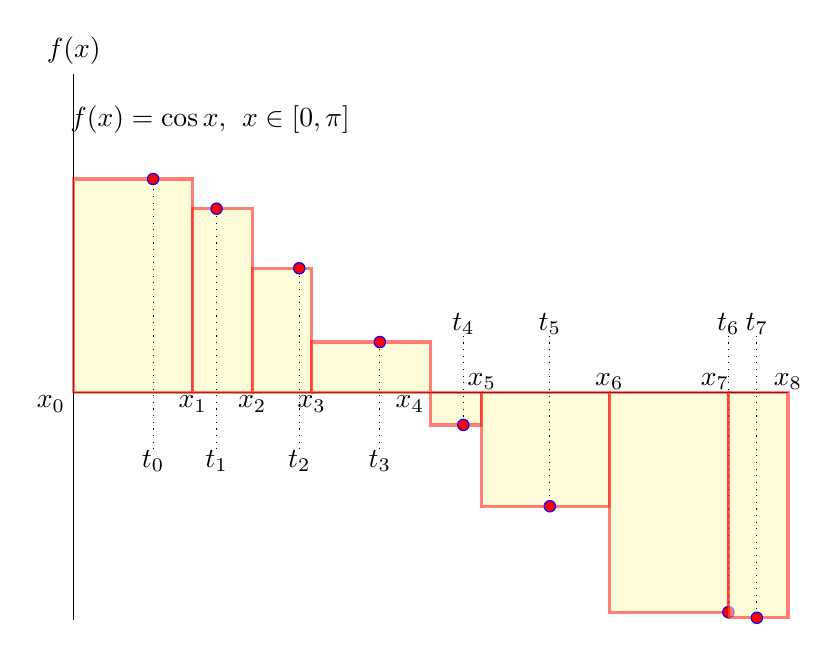
\begin{tikzpicture}[scale=\textwidth/4.2cm]
    % title and axes
    \node at (0.6, 1.2) {$f(x)=\cos x, \hspace{4pt} x \in [0, \pi]$};
    \draw (0, 0) -- (pi, 0);
    \draw (0, 0) -- (0, 1.4)
        node[above] {$f(x)$};
    \draw (0, 0) -- (0, -1);
    % graph
    \draw[black, very thick] plot[smooth] file {integrals_of_functions/python_generated_tables/cos_0_pi_riemann_sum.table};
    \draw[red, very thick, fill=yellow!30, opacity=0.5] (0, 0) 
        -- (pi/6, 0)
        -- (pi/6, {cos(pi/9 r)})
        -- (0, {cos(pi/9 r)})
        -- (0, 0);
    \node at (-0.1, -0.05) {$x_{0}$};
    \node at (pi/9, -0.3) {$t_{0}$};
    \node at (pi/6, -0.05) {$x_{1}$};
    \draw[black, dotted] (pi/9, -0.25) -- (pi/9, {cos(pi/9 r)});
    \draw[blue, fill=red] (pi/9, {cos(pi/9 r)}) circle (.25mm);
    \draw[red, very thick, fill=yellow!30, opacity=0.5] (pi/6, 0) 
        -- (pi/4, 0)
        -- (pi/4, {cos(pi/5 r)})
        -- (pi/6, {cos(pi/5 r)})
        -- (pi/6, 0);
    \node at (pi/5, -0.3) {$t_{1}$};
    \node at (pi/4, -0.05) {$x_{2}$};
    \draw[black, dotted] (pi/5, -0.25) -- (pi/5, {cos(pi/5 r)});
    \draw[blue, fill=red] (pi/5, {cos(pi/5 r)}) circle (.25mm);
    \draw[red, very thick, fill=yellow!30, opacity=0.5] (pi/4, 0) 
        -- (pi/3, 0)
        -- (pi/3, {cos(12*pi/38 r)})
        -- (pi/4, {cos(12*pi/38 r)})
        -- (pi/4, 0);
    \node at (12*pi/38, -0.3) {$t_{2}$};
    \node at (pi/3, -0.05) {$x_{3}$};
    \draw[black, dotted] (12*pi/38, -0.25) -- (12*pi/38, {cos(12*pi/38 r)});
    \draw[blue, fill=red] (12*pi/38, {cos(12*pi/38 r)}) circle (.25mm);
    \draw[red, very thick, fill=yellow!30, opacity=0.5] (pi/3, 0) 
        -- (pi/2, 0)
        -- (pi/2, {cos(12*pi/28 r)})
        -- (pi/3, {cos(12*pi/28 r)})
        -- (pi/3, 0);
    \node at (12*pi/28, -0.3) {$t_{3}$};
    \node at (8*pi/17, -0.05) {$x_{4}$};
    \draw[black, dotted] (12*pi/28, -0.25) -- (12*pi/28, {cos(12*pi/28 r)});
    \draw[blue, fill=red] (12*pi/28, {cos(12*pi/28 r)}) circle (.25mm);
    \draw[red, very thick, fill=yellow!30, opacity=0.5] (pi/2, 0) 
        -- (4*pi/7, 0)
        -- (4*pi/7, {cos(6*pi/11 r)})
        -- (pi/2, {cos(6*pi/11 r)})
        -- (pi/2, 0);
    \node at (6*pi/11, 0.3) {$t_{4}$};
    \node at (4*pi/7, 0.05) {$x_{5}$};
    \draw[black, dotted] (6*pi/11, 0.25) -- (6*pi/11, {cos(6*pi/11 r)});
    \draw[blue, fill=red] (6*pi/11, {cos(6*pi/11 r)}) circle (.25mm);
    \draw[red, very thick, fill=yellow!30, opacity=0.5] (4*pi/7, 0) 
        -- (3*pi/4, 0)
        -- (3*pi/4, {cos(2*pi/3 r)})
        -- (4*pi/7, {cos(2*pi/3 r)})
        -- (4*pi/7, 0);
    \node at (2*pi/3, 0.3) {$t_{5}$};
    \node at (3*pi/4, 0.05) {$x_{6}$};
    \draw[black, dotted] (2*pi/3, 0.25) -- (2*pi/3, {cos(2*pi/3 r)});
    \draw[blue, fill=red] (2*pi/3, {cos(2*pi/3 r)}) circle (.25mm);
    \draw[red, very thick, fill=yellow!30, opacity=0.5] (3*pi/4, 0) 
        -- (11*pi/12, 0)
        -- (11*pi/12, {cos(11*pi/12 r)})
        -- (3*pi/4, {cos(11*pi/12 r)})
        -- (3*pi/4, 0);
    \node at (11*pi/12, 0.3) {$t_{6}$};
    \node at (44*pi/49, 0.05) {$x_{7}$};
    \draw[black, dotted] (11*pi/12, 0.25) -- (11*pi/12, {cos(11*pi/12 r)});
    \draw[blue, fill=red] (11*pi/12, {cos(11*pi/12 r)}) circle (.25mm);
    \draw[red, very thick, fill=yellow!30, opacity=0.5] (11*pi/12, 0) 
        -- (pi, 0)
        -- (pi, {cos(22*pi/23 r)})
        -- (11*pi/12, {cos(22*pi/23 r)})
        -- (11*pi/12, 0);
    \node at (22*pi/23, 0.3) {$t_{7}$};
    \node at (pi, 0.05) {$x_{8}$};
    \draw[black, dotted] (22*pi/23, 0.25) -- (22*pi/23, {cos(22*pi/23 r)});
    \draw[blue, fill=red] (22*pi/23, {cos(22*pi/23 r)}) circle (.25mm);
\end{tikzpicture}
}
\begin{align*}
    &\text{The approximation can be computed with} \hspace{20pt} \sum_{i=0}^{7} f(t_{i})(x_{i+1} - x_{i})
\end{align*}
Taking a partition with uncountable infinitely many points between $0$ and $1$ is the key to computing the integral. The rectangles seen in this example each have an area: base times height. The difference $(x_{i+1} - x_{i})$ for each $i$ represents the base, while the function value at $t_{i}$ for each $i$ represents the height. So, the integral of our function $f$ ---the value of which we will discuss shortly--- can be expressed as the limit 
\begin{align*}
    \lim_{n \longrightarrow \infty} \sum_{i=0}^{n-1} \cos(t_{i}) (x_{i+1} - x_{i}) = \int_{0}^{1} \cos x dx = \sin x \hspace{4pt} x \in [0, 1]
\end{align*}
\label{integral_of_cosine}
\end{example}

\begin{theorem}
A function $f$ continuous on $[a, b]$ or continuous at all but a finite number of points along $[a, b]$ is integrable on $[a, b]$.
\label{monotone_continuous_functions_are_integrable}
\end{theorem}

Integration on the continuous functions mentioned in Theorem \ref{monotone_continuous_functions_are_integrable} will more times than not require us to use something referred to as antidifferentiation, as opposed to the computation of sums, using a result known as The Fundamental Theorem of Calculus, which we will get to later. For now, let's simply practice antidifferentiation on continuous functions and explore some properties of the Riemann integral. 

\begin{example}
The function $f(x) = \cos x$ is continuous on $[0, 1]$. Thus, for Example \ref{integral_of_cosine}, the antiderivative of $f$ is $g(x) = \sin x$.
\end{example}

\begin{example}
Take $f(x) = 1$ on some arbitrary domain $D$. The form of the integral on $f$ along this non-explicitly defined domain $D$ is referred to as the indefinite form of the integral. Meaning, the function domain is not bounded above or below by any specific real numbers. We will later discuss the difference between this indefinite form and what is known as the definite form of an integral, which we used in Example \ref{integral_of_cosine}. The domain is explicitly defined and bounded for cosine in that example, whereas the domain for $f$ in this example is not defined at all. More on this, later. In taking either form of the integral on a function $f$, the first question you should always ask yourself:
\begin{align*}
    &\text{The derivative of which function $g$ is equal to} \hspace{4pt} f?\\[2ex]
    &\text{Meaning, what is $g$, when} \hspace{4pt} \dfrac{dg}{dx} = f(x) \hspace{4pt} \text{?}
\end{align*}
Once you find $g$, \textbf{THAT} is the integral of $f$. With the indefinite form, we must consider the crucial detail of a real number (constant) as being part of the expression for our function $g$. Particularly, for our example, we know
\begin{align*}
f(x) = 1 \hspace{20pt} f(x) = 1 + 0
\end{align*}
and we know that the derivative of a constant is $0$ and the derivative of $x$ is $1$. So, when searching for the indefinite integral $g$, we not only must consider the `kernel' (the main part) of the function $f$, which in our case is $1$, we must also consider the implied $0$. 
Continuing with our example:
\begin{align*}
    \text{we know that} \hspace{20pt} \dfrac{d}{dx} (x+c) = \dfrac{d}{dx} x + \dfrac{d}{dx} c = 1 + 0 = 1 \hspace{20pt} \text{where} \hspace{4pt} c \in \mathbb{R}
\end{align*}
So, we have that $g(x) = x+c$, because $\dfrac{dg}{dx} = \dfrac{d}{dx}(x+c) = 1 + 0 = 1 = f(x)$. Additionally, because $f$ is continuous on $D$, we call $g$ an antiderivative of $f$. Thus, we have the indefinite integral
\begin{align*}
    g(x) = \int_{D} f(x)dx = \int_{D} 1 dx = x + c \hspace{20pt} \text{where $D$ is the domain of the function}
\end{align*}
which also happens to be an antiderivative. We could represent this integral without the $1$ under the integral sign, as follows
\begin{align*}
    g(x) = \int_{D} dx = x+c
\end{align*}
\end{example}

\begin{example}
Let's take the integral of $f(x) = x$. We know 
\begin{align*}
    \dfrac{d}{dx} \Big(\dfrac{x^{2}}{2} + c \Big) = \dfrac{d}{dx} \dfrac{x^{2}}{2} + \dfrac{d}{dx} c = \dfrac{2x}{2} + 0 = x
\end{align*}
So, $g(x) = \dfrac{x^{2}}{2} + c$ is the indefinite integral of $f$ and it also happens to be an antiderivative of $f$, since $f$ is continuous on $D$. The results are summarized below.
\begin{align*}
    \int_{D} f(x)dx = \int_{D} x dx  =  \dfrac{x^{2}}{2} + c = g(x)
\end{align*}
\end{example}

\begin{exercise}
Find the indefinite integral of the following
\begin{align*}
    f(x) = x^{n} \hspace{20pt} \text{where $n$ is a positive number} 
\end{align*}
\end{exercise}

\begin{exercise}
Find the indefinite integral of the following
\begin{align*}
    f(x) = x^{-n} \hspace{20pt} \text{where $n$ is a positive number}
\end{align*}
\end{exercise}

\begin{exercise}
Find the indefinite integral of the following
\begin{align*}
    f(x) = e^{x}
\end{align*}
\end{exercise}

\begin{exercise}
Find the indefinite integral of the following
\begin{align*}
    f(x) = \cos x
\end{align*}
\end{exercise}

\begin{exercise}
Find the indefinite integral of the following
\begin{align*}
    f(x) = \sin x
\end{align*}
\end{exercise}

\begin{theorem}
Following are some of the basic properties of the Riemann integral
\begin{align*}
    &\int_{D} c f(x) dx = c \int_{D} f(x) dx \hspace{20pt} \text{where} \hspace{4pt} c \in \mathbb{R}\\[2ex]
    &\int_{D} (f(x) + g(x)) dx = \int_{D} f(x) dx + \int_{D} g(x) dx\\[2ex]
    &\int_{D} (f(x) - g(x)) dx = \int_{D} f(x) dx - \int_{D} g(x) dx\\[2ex]
    &\text{If} \hspace{4pt} f(x) \geq 0 \hspace{4pt} \text{for all $x \in D$} \hspace{20pt} \text{then} \hspace{20pt} \int_{D} f(x) dx \geq 0\\[2ex]
    &\text{If} \hspace{4pt} f(x) \leq g(x) \hspace{4pt} \text{for all $x \in D$} \hspace{20pt} \text{then} \hspace{20pt} \int_{D} f(x) dx \leq \int_{D} g(x) dx
\end{align*}
\end{theorem}

\begin{exercise}
Find the indefinite integral of the following
\begin{align*}
    f(x) = 1 + 3x
\end{align*}
\end{exercise}

\begin{exercise}
Find the indefinite integral of the following
\begin{align*}
    f(x) = x^{2} + 2x - 5
\end{align*}
\end{exercise}

\begin{exercise}
Find the indefinite integral of the following
\begin{align*}
    f(x) = 2 - x^{2}
\end{align*}
\end{exercise}

\begin{exercise}
Find the indefinite integral of the following
\begin{align*}
    f(x) = 1 + 2x^{3}
\end{align*}
\end{exercise}

\begin{exercise}
Find the indefinite integral of the following
\begin{align*}
    f(x) = \dfrac{1}{2}x - 1
\end{align*}
\end{exercise}

\begin{exercise}
Find the indefinite integral of the following
\begin{align*}
    f(x) = 3 - 2x
\end{align*}
\end{exercise}

\newpage
\section{The Fundamental Theorem of Calculus}

\begin{theorem}
For function $f$ as described in Theorem \ref{monotone_continuous_functions_are_integrable}, we have the indefinite integral of $f$ represented as
\begin{align*}
    g(x) = \int_{a}^{x} f(t) dt \hspace{20pt} x \in [a, b]
\end{align*}
where $a$ is referred to as a basepoint. On the interval $[a, b]$, we have $g$ is continuous, and on the interval $(a, b)$, save for possibly finitely many points, we have $g$ is differentiable, with
\begin{align*}
    g^{'}(z) = f(z) \hspace{20pt} \text{for all} \hspace{4pt} z \in (a, b) \hspace{20pt} \text{save possibly finitely many points where $f$ is discontinuous}
\end{align*}
We refer to this as The Fundamental Theorem of Calculus I.\\[1ex]
When $f$ is continuous on the domain $[a, b]$, we call $g$ an antidervative of $f$. \label{FTC_1}
\end{theorem}

\begin{theorem}
For function $f$ as described in Theorem \ref{monotone_continuous_functions_are_integrable}, we have 
\begin{align*}
    g(b) - g(a) = \int_{a}^{b} f(x) dx \hspace{20pt} x \in [a, b]
\end{align*}
where $g$ is continuous on $[a, b]$. Also, $g$ is differentiable on $(a, b)$, save for finitely many points, with
\begin{align*}
    g^{'}(x) = f(x) \hspace{20pt} \text{for all} \hspace{4pt} x \in (a, b) \hspace{20pt} \text{save for possibly finitely many points where $f$ is discontinuous}
\end{align*}
We refer to this as The Fundamental Theorem of Calculus II.\\[1ex]
When $f$ is continuous on $[a, b]$, $g$ is an antiderivative of $f$.
\end{theorem}

\begin{exercise}
Find the definite integral of the following
\begin{align*}
    f(x) = 1 + 3x \hspace{20pt} x \in [-1, 5]
\end{align*}
\end{exercise}

\begin{exercise}
Find the definite integral of the following
\begin{align*}
    f(x) = x^{2} + 2x - 5 \hspace{20pt} x \in [1, 4]
\end{align*}
\end{exercise}

\begin{exercise}
Find the definite integral of the following
\begin{align*}
    f(x) = 2 - x^{2} \hspace{20pt} x \in [0, 2]
\end{align*}
\end{exercise}

\begin{exercise}
Find the definite integral of the following
\begin{align*}
    f(x) = 1 + 2x^{3} \hspace{20pt} x \in [0, 5]
\end{align*}
\end{exercise}

\begin{exercise}
Find the definite integral of the following
\begin{align*}
    f(x) = \dfrac{1}{2}x - 1 \hspace{20pt} x \in [0, 3]
\end{align*}
\end{exercise}

\begin{exercise}
Find the definite integral of the following
\begin{align*}
    f(x) = 3 - 2x \hspace{20pt} x \in [-1, 3]
\end{align*}
\end{exercise}

\begin{theorem}
Following are more of the basic properties of the Riemann integral
\begin{align*}
    &\text{If} \hspace{4pt} f(x) \geq 0 \hspace{4pt} \text{for all $x \in D$} \hspace{20pt} \text{then} \hspace{20pt} \int_{D} f(x) dx \geq 0\\[2ex]
    &\text{If} \hspace{4pt} f(x) \leq g(x) \hspace{4pt} \text{for all $x \in D$} \hspace{20pt} \text{then} \hspace{20pt} \int_{D} f(x) dx \leq \int_{D} g(x) dx 
\end{align*}
\end{theorem}

\begin{example}
In many situations, we could make use of a substitution method to simplify our process of integration. Take the following
\begin{align*}
    f(x) = \sqrt{2x + 1} \hspace{20pt} x \in [0, 4]
\end{align*}
We have the definite integral represented as 
\begin{align*}
    g(x) = \int_{0}^{4} \sqrt{2x + 1} dx
\end{align*}
To make the job of integration easier, we could set $u(x) = 2x + 1$. This would imply the following
\begin{align*}
    \dfrac{du}{dx} = 2 \hspace{10pt} \Longleftrightarrow \hspace{10pt} \dfrac{du}{2} = dx \hspace{20pt} \text{and} \hspace{20pt} u(x) \in [1, 9]
\end{align*}
Thus, the integral can be rewritten from this substitution as
\begin{align*}
    g(x) = \int_{1}^{9} \dfrac{1}{2}\sqrt{u(x)} du = \int_{1}^{9} \dfrac{1}{2} \hspace{4pt} (u(x))^{1/2} \hspace{4pt} du = \dfrac{1}{3} (u(x))^{3/2} \hspace{20pt} u(x) \in [1, 9]
\end{align*}
The right hand side of the equality evaluates to $26/3$. However, if one wishes to revert back to expressions in terms of $x$, as opposed to $u(x)$, the numerically computation will be the same.
\begin{align*}
    g(x) &= \int_{1}^{9} \dfrac{1}{2}\sqrt{u(x)} du = \dfrac{1}{3} (u(x))^{3/2} \hspace{20pt} u(x) \in [1, 9]\\[2ex]
    &= \dfrac{1}{3} (\sqrt{2x + 1})^{3/2} \hspace{20pt} x \in [0, 4]\\[2ex]
    &= \dfrac{1}{3} (\sqrt{2(4) + 1})^{3/2} - \dfrac{1}{3} (\sqrt{2(0) + 1})^{3/2} = \dfrac{26}{3}
\end{align*}
\end{example}

\begin{example}
Consider the following indefinite integral
\begin{align*}
    g(x) = \int_{D} \cos^{3} x \sin x dx
\end{align*}
It looks tough, but with a tool referred to as \textbf{U-Substitution}, we got this. Define
\begin{align*}
    u(x) = \cos x
\end{align*}
By differentiating $u$ with respect to $x$, we get
\begin{align*}
    \dfrac{du}{dx} = -\sin x \hspace{20pt} \Longleftrightarrow \hspace{20pt} -du = \sin x dx
\end{align*}
Thus, our indefinitie integral becomes
\begin{align*}
    g(x) &= \int_{D} -(u(x))^{3} du\\[2ex]
    &= \hspace{4pt} -\dfrac{1}{4} (u(x))^{4} + c\\[2ex]
    &= \hspace{4pt} -\dfrac{1}{4} \cos^{4} x + c
\end{align*}
\end{example}

\begin{exercise}
Find the indefinite integral of the following 
\begin{align*}
    f(x) = \dfrac{\sec^{2} \Big(\dfrac{1}{x}\Big)}{x^{2}}
\end{align*}
\end{exercise}

\begin{exercise}
Find the indefinite integral of the following 
\begin{align*}
    f(x) = x \sin(x^{2})
\end{align*}
\end{exercise}

\begin{exercise}
Find the indefinite integral of the following 
\begin{align*}
    f(x) = \dfrac{x}{(x^{2} + 1)^{2}}
\end{align*}
\end{exercise}

\begin{exercise}
Find the indefinite integral of the following 
\begin{align*}
    f(x) = e^{x} \sin (e^{x})
\end{align*}
\end{exercise}

\begin{exercise}
Find the indefinite integral of the following 
\begin{align*}
    f(x) = \dfrac{x}{x^{2} + 1}
\end{align*}
\end{exercise}

\begin{exercise}
Find the indefinite integral of the following 
\begin{align*}
    f(x) = \dfrac{(\ln x)^{2}}{x}
\end{align*}
\end{exercise}

\begin{exercise}
Find the indefinite integral of the following 
\begin{align*}
    f(x) = (1 + \tan x)^{5} \sec^{2} x
\end{align*}
\end{exercise}

\begin{exercise}
Find the indefinite integral of the following 
\begin{align*}
    f(x) = e^{x} \sin (e^{x})
\end{align*}
\end{exercise}

\begin{exercise}
Find the indefinite integral of the following 
\begin{align*}
    f(x) = \dfrac{\sin(\ln x)}{x}
\end{align*}
\end{exercise}

\begin{exercise}
Find the indefinite integral of the following 
\begin{align*}
    f(x) = \dfrac{\cos x}{\sin^{2} x}
\end{align*}
\end{exercise}

\begin{exercise}
Find the indefinite integral of the following 
\begin{align*}
    f(x) = \sqrt{\cot x} \csc^{2} x
\end{align*}
\end{exercise}

\begin{exercise}
Find the indefinite integral of the following 
\begin{align*}
    f(x) = \sec^{3} x \tan x
\end{align*}
\end{exercise}

\begin{exercise}
Find the indefinite integral of the following 
\begin{align*}
    f(x) = \dfrac{1+x}{1 + x^{2}}
\end{align*}
\end{exercise}

\begin{exercise}
Find the indefinite integral of the following 
\begin{align*}
    f(x) = \dfrac{x^{2}}{\sqrt{1 - x}}
\end{align*}
\end{exercise}

\begin{exercise}
Find the indefinite integral of the following 
\begin{align*}
    f(x) = \dfrac{x}{\sqrt[\leftroot{2}\uproot{2}4]{x + 2}}
\end{align*}
\end{exercise}

\begin{exercise}
Find the indefinite integral of the following 
\begin{align*}
    f(x) = x^{3} \sqrt{x^{2} + 1}
\end{align*}
\end{exercise}

\begin{exercise}
Find the definite integral of the following 
\begin{align*}
    f(x) = x^{2} (1 + 2x^{3})^{5} \hspace{20pt} x \in [0, 1]
\end{align*}
\end{exercise}

\begin{exercise}
Find the definite integral of the following 
\begin{align*}
    f(x) = \dfrac{e^{1/x}}{x^{2}} \hspace{20pt} x \in [1, 2]
\end{align*}
\end{exercise}

\begin{exercise}
Find the indefinite integral of the following
\begin{align*}
    f(x) = \tan x
\end{align*}
\end{exercise}

\begin{exercise}
Find the indefinite integral of the following
\begin{align*}
    f(x) = \sec x
\end{align*}
\end{exercise}

\begin{example}
Using Theorem \ref{FTC_1}, we can find the derivative of an indefinite integral. Take the following
\begin{align*}
    \int_{1}^{x^{4}} \sec t dt
\end{align*}
The function under the integral sign is continuous. Additionally, we have $x^{4}$ as our upper bound on the integral sign. Let's define $u(x) = x^{4}$. Our function $g$ can now be written as 
\begin{align*}
    g(x) = (v \circ u)(x) = \int_{1}^{u(x)} \sec t dt
\end{align*}
By The Fundamental Theorem of Calculus I, along with The Chain Rule 
\begin{align*}
    \dfrac{dg}{dx} &= v^{'}(u(x)) \cdot u^{'}(x)\\[2ex] 
    &= \dfrac{d}{du} \Big( \int_{1}^{u(x)} \sec t dt \Big) \dfrac{du}{dx}\\[2ex]
    &= ( \sec u(x) ) \cdot 4x^{3}\\[2ex]
    &= 4x^{3} \sec x^{4} 
\end{align*}
\end{example}

\begin{exercise}
Find the derivative of $g$.
\begin{align*}
    g(x) = \int_{1}^{x} \dfrac{1}{t^{3} + 1} dt
\end{align*}
\end{exercise}

\begin{exercise}
Find the derivative of $g$.
\begin{align*}
    g(x) = \int_{2}^{x} t^{2} \sin t dt
\end{align*}
\end{exercise}

\begin{note}
\begin{align*}
    \int_{b}^{a} f(x) dx = -\int_{a}^{b} f(x) dx \hspace{20pt} a, b \in \mathbb{R}
\end{align*}
\end{note}

\begin{exercise}
Find the derivative of $g$.
\begin{align*}
    g(x) = \int_{x}^{\pi} \sqrt{1 + \sec t} dt
\end{align*}
\end{exercise}

\begin{exercise}
Find the derivative of $g$.
\begin{align*}
    g(x) = \int_{2}^{1/x} \arctan t dt
\end{align*}
\end{exercise}

\begin{exercise}
Find the derivative of $g$.
\begin{align*}
    g(x) = \int_{1}^{\cos x} (1 + t^{2})^{10} dt
\end{align*}
\end{exercise}

\begin{exercise}
Find the derivative of $g$.
\begin{align*}
    g(x) = \int_{e^{x}}^{0} \sin^{3} t dt
\end{align*}
\end{exercise}

\newpage
\section{Integration by Parts}

\begin{theorem}
Let $u$, $v$ be differentiable on $[a, b]$ and let $f = u^{'}$ and $g = v^{'}$ be Riemann integrable. Then the following holds
\begin{align*}
    \int_{a}^{b} ug = uv \Big|_{a}^{b} - \int_{a}^{b} vf
\end{align*}
\begin{proof}
By the product rule
\begin{align*}
    (uv)^{'} = fv + ug = vf + ug
\end{align*}
We know differentiable functions are Riemann integrable, and we are told that $f$ and $g$ are integrable. Thus,
\begin{align*}
    \int_{a}^{b} (uv)^{'} &= \int_{a}^{b} vf + \int_{a}^{b} ug\\[2ex]
    &\Longleftrightarrow\\[2ex]
    uv \Big|_{a}^{b} &= \int_{a}^{b} vf + \int_{a}^{b} ug\\[2ex] 
    &\Longleftrightarrow\\[2ex]
    \int_{a}^{b} ug &= uv \Big|_{a}^{b} - \int_{a}^{b} vf\\[2ex]
    \int_{a}^{b} u dv &= uv \Big|_{a}^{b} - \int_{a}^{b} v du
\end{align*}
\end{proof}
We refer to this integration technique as Integration by Parts.
\end{theorem}

\begin{example}
We find the following integral
\begin{align*}
    \int_{D} \ln x dx
\end{align*}
by defining the following
\begin{align*}
    &u(x) = \ln x \hspace{20pt} \Longrightarrow \hspace{20pt} \dfrac{du}{dx} = \dfrac{1}{x} \hspace{20pt} \Longleftrightarrow \hspace{20pt} du = \dfrac{dx}{x}\\[2ex]
    &dv = dx \hspace{20pt} \Longrightarrow \hspace{20pt} v(x) = \int_{D} dv = \int_{D} dx = x
\end{align*}
Using Integration by Parts, with $c_{0}, c_{1} \in \mathbb{R}$ this gives us the following setup
\begin{align*}
    \int_{D} \ln x dx = \int_{D} u(x) dv = u(x)v(x) - \int_{D} v(x) du = \ln x \cdot x + c_{0} - \int_{D} x \dfrac{dx}{x} = \ln x \cdot x + c_{0} - x + c_{1}
\end{align*}
We now combine our constants into one constant $c$ for the final result
\begin{align*}
    \int_{D} \ln x dx = x \ln x - x + c
\end{align*}
\end{example}

\begin{exercise}
Find the indefinite integral of the following
\begin{align*}
    f(x) = x^{2} \ln x
\end{align*}
\end{exercise}

\begin{exercise}
Find the indefinite integral of the following
\begin{align*}
    f(x) = x \cos x
\end{align*}
\end{exercise}

\begin{exercise}
Find the indefinite integral of the following
\begin{align*}
    f(x) = x \cos(mx) \hspace{20pt} m \in \mathbb{R}
\end{align*}
\end{exercise}

\begin{exercise}
Find the indefinite integral of the following
\begin{align*}
    f(x) = x^{2} e^{x}
\end{align*}
\end{exercise}

\begin{exercise}
Find the indefinite integral of the following
\begin{align*}
    f(x) = \sin x \cdot e^{x}
\end{align*}
\end{exercise}

\begin{exercise}
Find the indefinite integral of the following
\begin{align*}
    f(x) = \arctan x
\end{align*}
\end{exercise}

\begin{exercise}
Find the indefinite integral of the following
\begin{align*}
    f(x) = x \sec^{2} x
\end{align*}
\end{exercise}

\begin{exercise}
Find the indefinite integral of the following
\begin{align*}
    f(x) = x \cdot 2^{x}
\end{align*}
\end{exercise}

\begin{exercise}
Find the indefinite integral of the following
\begin{align*}
    f(x) = e^{-x} \cos(2x)
\end{align*}
\end{exercise}

\begin{exercise}
Find the definite integral of the following
\begin{align*}
    f(x) = \dfrac{\ln x}{x^{2}} \hspace{20pt} x \in [1, 2]
\end{align*}
\end{exercise}

\begin{exercise}
Find the definite integral of the following
\begin{align*}
    f(x) = \dfrac{x}{e^{2x}} \hspace{20pt} [0, 1]
\end{align*}
\end{exercise}

\begin{exercise}
Find the definite integral of the following
\begin{align*}
    f(x) = \arccos x \hspace{20pt} \Big[0, \hspace{4pt} \dfrac{1}{2}\Big]
\end{align*}
\end{exercise}

\begin{note}
There are times when multiple integration approaches/techniques make integration easier.
\end{note}

\begin{exercise}
Find the indefinite integral of the following
\begin{align*}
    f(x) = x^{3} \cos(x^{2}) \hspace{20pt} \Big[\sqrt{\dfrac{\pi}{2}}, \hspace{4pt} \sqrt{\pi} \Big]
\end{align*}
\end{exercise}

\begin{exercise}
Find the definite integral of the following
\begin{align*}
    f(x) = e^{\cos x} \sin(2x) \hspace{20pt} [0, \pi]
\end{align*}
\end{exercise}

\begin{exercise}
Find the indefinite integral of the following
\begin{align*}
    f(x) = \cos \sqrt{x}
\end{align*}
\end{exercise}

\newpage
\section{Trigonometric Integrals}

\begin{recall}
We will use the following trigonometric identities, along with previously discussed techniques, to solve the integrals within this section.
\begin{align*}
    &1 = \cos^{2} x + \sin^{2} x\\[2ex]
    &\cos(2x) = \cos^{2} x - \sin^{2} x\\[2ex]
    &\sin(2x) = 2\sin x \cos x
\end{align*}
\end{recall}

\begin{exercise}
Find the definite integral of the following
\begin{align*}
    f(x) = \cos x \hspace{20pt} x \in \Big[0, \hspace{4pt} \dfrac{\pi}{2} \Big]
\end{align*}
\end{exercise}

\begin{exercise}
Find the definite integral of the following
\begin{align*}
    f(x) = \sin^{2}(2x) \hspace{20pt} x \in \Big[0, \hspace{4pt} \dfrac{\pi}{2} \Big]
\end{align*}
\end{exercise}

\begin{exercise}
Find the indefinite integral of the following
\begin{align*}
    f(x) = \sin^{3} x \cos^{2} x
\end{align*}
\end{exercise}

\begin{exercise}
Find the definite integral of the following
\begin{align*}
    f(x) = \sin^{2} x \cos^{2} x \hspace{20pt} x \in \Big[0, \dfrac{\pi}{2} \Big]
\end{align*}
\end{exercise}

\begin{exercise}
Find the indefinite integral of the following
\begin{align*}
    f(x) = x \cos^{2} x
\end{align*}
\end{exercise}

\begin{exercise}
Find the indefinite integral of the following
\begin{align*}
    f(x) = \sec^{2} x \tan x
\end{align*}
\end{exercise}

\begin{exercise}
Find the indefinite integral of the following
\begin{align*}
    f(x) = \tan^{2} x 
\end{align*}
\end{exercise}

\begin{exercise}
Find the definite integral of the following
\begin{align*}
    f(x) = \sec^{4} x \tan^{4} x \hspace{20pt} x \in \Big[0, \dfrac{\pi}{4} \Big]
\end{align*}
\end{exercise}

\begin{exercise}
Find the indefinite integral of the following
\begin{align*}
    f(x) = \tan^{3} x \sec x
\end{align*}
\end{exercise}

\begin{exercise}
Find the indefinite integral of the following
\begin{align*}
    f(x) = \dfrac{\sin x}{\cos^{3} x}
\end{align*}
\end{exercise}

\begin{exercise}
Find the definite integral of the following
\begin{align*}
    f(x) = \cot^{2} x \hspace{20pt} \Big[\dfrac{\pi}{6}, \dfrac{\pi}{2}\Big]
\end{align*}
\end{exercise}

\begin{exercise}
Find the indefinite integral of the following
\begin{align*}
    f(x) = \csc x
\end{align*}
\end{exercise}

\begin{exercise}
Find the definite integral of the following
\begin{align*}
    f(x) = \csc^{3} x \hspace{20pt} \Big[\dfrac{\pi}{6}, \dfrac{\pi}{3}\Big]
\end{align*}
\end{exercise}

\newpage
\section{Integration by Partial Fractions}

\begin{recall}
We call the quotient of two polynomials a rational function. Let $p$ and $q$ be polynomials. Then $r$, with the following definition, is a rational function
\begin{align*}
    r(x) = \dfrac{p(x)}{q(x)}
\end{align*}
In this section, we will deal with rational functions, some of which may require long division. Following are a few details about which forms of rational functions we are likely to encounter within this section, as well as some examples of how to break these forms down into partial fractions that are relatively easier to integrate.
\end{recall}

\begin{note}
The rational functions that we will deal with in this section may include within their denominators some of the following:
\begin{itemize}
    \item Distinct, linear factors
    \item Non-distinct, linear factors
    \item Distinct, irreducible, quadratic factors
    \item Non-distinct, irreducible, quadratic factors
\end{itemize}
\label{four_cases_for_partial_fractions}
\end{note}

\begin{recall}
Long division of polynomials takes place when the degree of the polynomial in the denominator is less than the degree of the polynomial in the numerator.
\end{recall}

\begin{example}
Let
\begin{align*}
    f(x) = \dfrac{x^{3} + x}{x - 1}
\end{align*}
Using an algorithm for long division of polynomials
\begin{align*}
\setstackgap{S}{1.5pt}
\stackMath\def\stackalignment{r}
\stackunder{
  x-1 \stackon[1pt]{\showdiv{x^{3} + \hspace{20pt} + x}}{x^{2} + x + 2}
}{
  \Shortstack[l]{{\underline{x^{3}-x^{2}}\ph{\hspace{10pt} + x}} \ph{x^{3}-}x^{2}+x {\ph{x^{3}-}\underline{x^{2}-x}} \ph{x^{3}-x^{2}-}2x {\ph{x^{3}-x^{2}-}\underline{2x}} 
   \ph{x^{3}-x^{2}-}0}
  }
\end{align*}
Thus,
\begin{align*}
    f(x) = \dfrac{x^{3} + x}{x - 1} = x^{2} + x + 2 + \dfrac{0}{x - 1} = x^{2} + x + 2
\end{align*}
\end{example}

\begin{example}
We wish to integrate the following function
\begin{align*}
    f(x) = \dfrac{x^{2} + 2x - 1}{2x^{3} + 3x^{2} - 2x}
\end{align*}
Our goal is to rewrite this rational function in one of the four forms mentioned in Note \ref{four_cases_for_partial_fractions}. Factoring the denominator, we get
\begin{align*}
    \dfrac{x^{2} + 2x - 1}{2x^{3} + 3x^{2} - 2x} = \dfrac{x^{2} + 2x - 1}{x(2x - 1)(x + 2)}
\end{align*}
We see that each linear factor in the denominator. We may now break the single fraction into multiple fractions, as follows
\begin{align*}
    \dfrac{x^{2} + 2x - 1}{x(2x - 1)(x + 2)} = \dfrac{a}{x} + \dfrac{b}{2x - 1} + \dfrac{c}{x + 2}
\end{align*}
Multiplying through by the factored denominator, we have
\begin{align*}
    (x(2x - 1)(x + 2)) \cdot \dfrac{x^{2} + 2x - 1}{x(2x - 1)(x + 2)} \hspace{4pt} &= \hspace{4pt} (x(2x - 1)(x + 2)) \cdot \Big(\dfrac{a}{x} + \dfrac{b}{2x - 1} + \dfrac{c}{x + 2} \Big)\\[2ex]
    &\Longleftrightarrow\\[2ex]
    x^{2} + 2x - 1 \hspace{4pt} &= \hspace{4pt} a(2x - 1)(x + 2) + bx(x + 2) + cx(2x - 1)
\end{align*}
After a bit of rearrangement, we get
\begin{align*}
    x^{2} + 2x - 1 \hspace{4pt} = (2a + b + 2c)x^{2} + (3a + 2b - c)x - 2a
\end{align*}
Now, we can set the coefficients for the polynomial on the left-hand side equal to the coefficients for the polynomial on the right-hand side
\begin{align*}
    1 &= 2a + b + 2c\\[2ex]
    2 &= 3a + 2b - c\\[2ex]
    -1 &= -2a
\end{align*}
Using our experience with systems of equations, we get
\begin{align*}
    a = \dfrac{1}{2} \hspace{20pt} b = \dfrac{1}{5} \hspace{20pt} c = -\dfrac{1}{10}
\end{align*}
giving us the resulting integral
\begin{align*}
    \int_{D} \dfrac{x^{2} + 2x - 1}{2x^{3} + 3x^{2} - 2x} dx &= \int_{D} \Big(\dfrac{1}{2} \cdot \dfrac{1}{x} + \dfrac{1}{5} \cdot \dfrac{1}{2x - 1} - \dfrac{1}{10} \cdot \dfrac{1}{x + 2}\Big) dx\\[2ex]
    &= \dfrac{1}{2}\int_{D} \dfrac{1}{x} dx \hspace{4pt} + \hspace{4pt} \dfrac{1}{5}\int_{D} \dfrac{1}{2x - 1} dx \hspace{4pt} - \hspace{4pt} \dfrac{1}{10}\int_{D} \dfrac{1}{x+2} dx\\[2ex]
    &= \dfrac{1}{2}\ln \lvert x \rvert + \dfrac{1}{10}\ln \lvert 2x - 1 \rvert - \dfrac{1}{10}\ln \lvert x + 2 \rvert + k
\end{align*}
where $k \in \mathbb{R}$
\end{example}

\begin{example}
The general form resulting from the breakdown of rational functions with (exclusively) distinct linear factors within the denominator is as follows
\begin{align*}
    f(x) = \frac{p(x)}{q(x)} &= \dfrac{p(x)}{(a_{1}x + b_{1})(a_{2}x + b_{2}) \cdots (a_{n-1}x + b_{n-1})(a_{n}x + b_{n})}\\[2ex]
    &= \dfrac{c_{1}}{a_{1}x + b_{1}} + \dfrac{c_{2}}{a_{2}x + b_{2}} + \cdots + \dfrac{c_{n-1}}{a_{n-1}x + b_{n-1}} + \dfrac{c_{n}}{a_{n}x + b_{n}}
\end{align*}
\end{example}

\begin{example}
As an example of how we may break a rational function down into multiple partial fractions, the denominator of which containing non-distinct linear factors, take
\begin{align*}
    f(x) = \dfrac{x^{4} - 2x^{2} + 4x + 1}{x^{3} - x^{2} - x + 1}
\end{align*}
Using long division, we can rewrite $f$ as follows
\begin{align*}
    f(x) = \dfrac{x^{4} - 2x^{2} + 4x + 1}{x^{3} - x^{2} - x + 1} = x + 1 + \dfrac{4x}{x^{3} - x^{2} - x + 1}
\end{align*}
Factoring the denominator of the resulting fractional portion of the rational function, we get
\begin{align*}
    f(x) = x + 1 + \dfrac{4x}{x^{3} - x^{2} - x + 1} = x + 1 + \dfrac{4x}{(x-1)^{2} (x+1)}
\end{align*}
Breaking this down to partial fractions, noting that $(x-1)$ occurs twice, we get
\begin{align*}
    f(x) = x + 1 + \dfrac{4x}{(x-1)^{2} (x+1)} = x + 1 + \dfrac{a}{x - 1} + \dfrac{b}{(x - 1)^{2}} + \dfrac{c}{x + 1}
\end{align*}
\end{example}

\begin{example}
The general form resulting from the breakdown of rational functions with (exclusively) repeating linear factors within the denominator is as follows
\begin{align*}
    f(x) = \dfrac{p(x)}{q(x)} &= \dfrac{p(x)}{(ax + b)^{n}}\\[2ex]
    &= \dfrac{c_{1}}{(ax + b)} + \dfrac{c_{2}}{(ax + b)^{2}} + \cdots \dfrac{c_{n-1}}{(ax + b)^{n-1}} + \dfrac{c_{n}}{(ax + b)^{n}}
\end{align*}
\end{example}

\begin{example}
As an example of how to break a rational function down into multiple partial functions, the denominator of which containing irreducible quadratic factors, take
\begin{align*}
    f(x) = \dfrac{x}{(x-2)(x^{2} + 1)(x^{2} + 4)}
\end{align*}
We can now take the function $f$ and rewrite it as multiple rationals, each with a single factor in its denominator
\begin{align*}
    f(x) &= \dfrac{x}{(x-2)(x^{2} + 1)(x^{2} + 4)}\\[2ex]
    &= \dfrac{a}{x-2} + \dfrac{bx + c}{x^{2} + 1} + \dfrac{dx + e}{x^{2} + 4}
\end{align*}
\end{example}

\begin{example}
The general form resulting from the breakdown of rational functions with (exclusively) distinct, irreducible quadratic factors within the denominator is as follows
\begin{align*}
    f(x) = \dfrac{p(x)}{q(x)} &= \dfrac{p(x)}{(a_{1}x^{2} + b_{1}x + c_{1}) \cdots (a_{n}x^{2} + b_{n}x + c)}\\[2ex]
    &= \dfrac{d_{1}x + e_{1}}{a_{1}x^{2} + b_{1}x + c_{1}} + \cdots + \dfrac{d_{n}x + e_{n}}{a_{n}x^{2} + b_{n}x + c_{n}}
\end{align*}
\end{example}

\begin{example}
As an example of how to break a rational function down into multiple partial functions, the denominator of which containing repeating, irreducible quadratic factors, take
\begin{align*}
    f(x) = \dfrac{x^{3} + x^{2} + 1}{x(x-1)(x^{2} + x + 1)(x^{2} + 1)^{3}}
\end{align*}
We can now take the function $f$ and rewrite it as multiple rationals, each with a single factor in its denominator
\begin{align*}
    f(x) &= \dfrac{x^{3} + x^{2} + 1}{x(x-1)(x^{2} + x + 1)(x^{2} + 1)^{3}}\\[2ex]
    &= \dfrac{a}{x} + \dfrac{b}{x-1} + \dfrac{cx + d}{x^{2} + x + 1} + \dfrac{ex + f}{x^{2} + 1} + \dfrac{gx + h}{(x^{2} + 1)^{2}} + \dfrac{ux + v}{(x^{2} + 1)^{3}}
\end{align*}
\end{example}

\begin{example}
The general form resulting from the breakdown of rational functions with (exclusively) repeating, irreducible quadratic factors within the denominator is as follows
\begin{align*}
    f(x) &= \dfrac{p(x)}{q(x)} = \dfrac{p(x)}{(ax^{2} + bx + c)^{n}}\\[2ex]
    &= \dfrac{c_{1}x + d_{1}}{ax^{2} + bx + c} + \dfrac{c_{2}x + d_{2}}{(ax^{2} + bx + c)^{2}} + \cdots + \dfrac{c_{n-1}x + d_{n-1}}{(ax^{2} + bx + c)^{n-1}} + \dfrac{c_{n}x + d_{n}}{(ax^{2} + bx + c)^{n}}
\end{align*}
\end{example}

\newpage
\section{Improper Integrals}